%-------------------------------------------------------------------------------
% yum_top_panel
%-------------------------------------------------------------------------------
%
% \file        yum_top_panel.tex
% \library     Documents
% \author      Chris Ahlstrom
% \date        2015-05-29
% \update      2017-09-03
% \version     $Revision$
% \license     $XPC_GPL_LICENSE$
%
%     Provides the Top Panel section of yoshimi-user-manual.tex.
%
%-------------------------------------------------------------------------------

\section{Top Panel}
\label{sec:top_panel}

   The \textsl{Yoshimi} top panel provides quick access to some major
   features of the application.
   The top panel is shown in
   \figureref{fig:yoshimi_main_screen}.

   Here are the major elements of the top panel.

   \begin{enumber}
      \item \textbf{Stop!}
      \item \textbf{Reset}
%     \item \textbf{Panel}
      \item \textbf{Mixer Panel}
%     \item \textbf{VirKbd}
      \item \textbf{Virtual Keybd}
      \item \textbf{Vectors}
      \item \textbf{Reports}
      \item \textbf{Key Shift}
      \item \textbf{Detune}
%     \item \textbf{Reset Detune}
      \item \textbf{Volume}
   \end{enumber}

   \setcounter{ItemCounter}{0}      % Reset the ItemCounter for this list.

   \itempar{Stop!}{top panel!stop all sound}
   Stop!
   This button causes \textsl{Yoshimi} to
   "Cease all sound immediately!"
   Useful when MIDI input suddenly stops due to a bug in the MIDI source.

   \itempar{Reset}{top panel!reset}
   Resets \textsl{Yoshimi} to its default state (when no default configuration
   files exist).  
   Or does it reset to the default loaded state (which the user may have saved
   earlier)?

   \itempar{Mixer Panel}{top panel!mixer panel}
   This button brings up a panel that shows a "mixer" view
   of all of the parts that have been created in the current
   state of \textsl{Yoshimi}.

   For the details of this panel,
   see \sectionref{subsec:mixer_panel_window}.

   \itempar{Virtual Keybd}{top panel!virtual keyboard}
   This button brings up the virtual keyboard, which is a way to enter
   MIDI information without a real MIDI keyboard. 
   It also provides a way to use the computer keyboard for faster
   playing.  See \sectionref{subsec:virtual_keyboard}.

   \itempar{Vectors}{top panel!vectors}
   Provides the recent new feature of vector control.  This has been moved moved
   to this button from the \textbf{Yoshimi} menu.  See
   \sectionref{subsec:vector_dialogs}.

   \itempar{Reports}{top panel!reports}
   This button is active only if reports are not going to
   \texttt{stdout}, by setting \textbf{Yoshimi / Settings / Main Settings / Send
   reports to:} to \textsl{Console Window}
   (see \sectionref{paragraph:menu_yoshimi_settings_main_settings} for this
   item.)
   When pressed, the \textsl{Yoshimi} console window is opened.

   \itempar{Key Shift}{top panel!key shift}
   Master Key Shift.
   This is the key-shift (transpose) that applies to all parts, in units of
   semitones.
   In recent versions of \textsl{Yoshimi}, this range has been extended.
   Also note that the master key shift can be set via the user-interface, the
   command-line, or (we suspect) by MIDI NRPN commands.

   Values: \texttt{-36 to 36, 0*}

   Also see the \textbf{Key Shift} item in 
   \sectionref{sec:bottom_panel} for more information.

   \itempar{Detune}{top panel!detune}
   Detune.  Provides a global fine detune functionality.
   The fine detune mapping to the knob values shown below is
   -64 to 63 cents.

   Values: \texttt{0 to 127, 64*} (float)

%  \itempar{Reset, Detune}{top panel!detune reset}
%  Reset detune.
%  Resets the overall detuning functionality of 
%  \textsl{Yoshimi} off.
%  Resets the global fine detune to 0.

   \itempar{Volume}{top panel!overall volume}
   Volume, Master Volume.
   Controls the overall volume of all sounds generated by
   \textsl{Yoshimi}.

   Values: \texttt{0 to 127, 90*}

\subsection{Mixer Panel Window}
\label{subsec:mixer_panel_window}
\index{Panel}

   The \textsl{Mixer Panel} button opens the mixer panel window, sometimes
   called the "Mixer" window.
   The mixer panel window provides a global view of the most important
   adjustable parameters of all of the defined parts.
   There are two views, a 2x8 view and a 2x16 view.
   See \figureref{fig:yoshimi_part_panel_2x8}, which
   shows the 2x8 view.

   The Panel Window allows one to edit some important part parameters
   (instrument/volume/panning/etc.) and it acts like a mixer. Also, this
   window shows VU-meters for each part.  To make a part the current part,
   left-click on its \textbf{Edit} button. To edit an instrument, right-click
   on the \textbf{Edit} button for that instrument.

   When using the JACK audio backend, parts can be individually routed or sent
   to the main L/R outputs, either by themselves, or working with the main Left
   and Right outputs at the same time.  This is controlled from the panel
   window, and the settings are saved with all the other parameters.

   The individual part outputs will have the part effects, and any
   \textbf{Insertion} effects that are linked to them, but not the
   \textbf{System} effects.
   Direct part outputs carry the part and insertion effects, but not system
   ones.

   \textsl{Yoshimi} used to register all parts with JACK by default, but that
   is a bit much now that 64 parts are available, so now \textsl{Yoshimi}
   uses an "on demand" model.

   In the mixer panel window one will see a field just above the
   \textbf{Edit} button.
   This field determines the audio destination on a part-by-part basis,
   defaulting to just the main L+R pair. The direct part outputs are only
   exposed on parts that are active, and have the destination set to either
   \textbf{part} or \textbf{both}.
   Once activated, they will remain in place for the entire session, even if
   the part is later disabled or routed to main only. This is so that other
   programs won't see links suddenly disappear, although they will become
   silent.  This setting is preserved in Yoshimi's patch sets and will be
   re-instated when next loaded.

\begin{figure}[H]
   \centering 
%  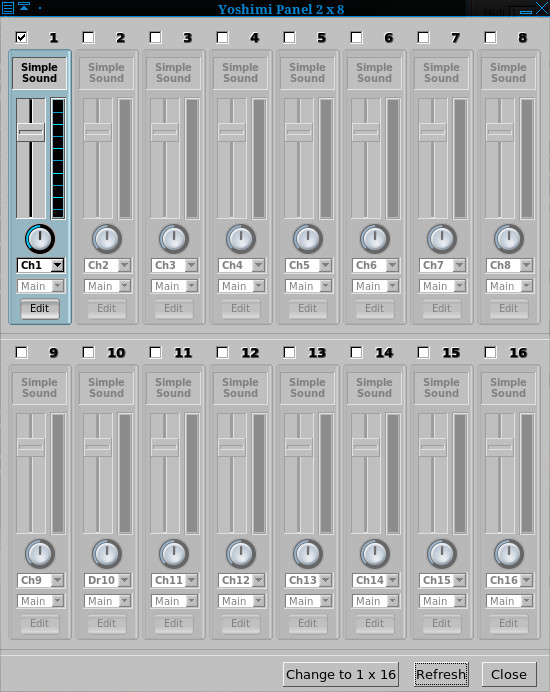
\includegraphics[scale=0.75]{top-panel/yoshimi-panel-2x8.jpg}
%  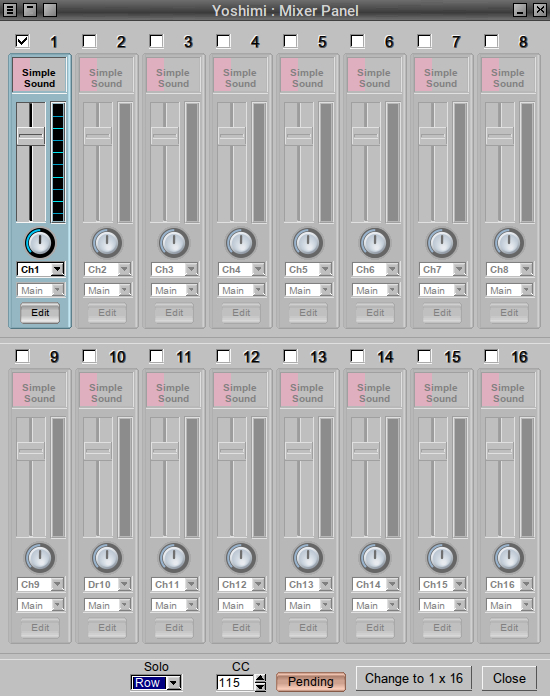
\includegraphics[scale=0.75]{top-panel/yoshimi-panel-2x8-1_5.jpg}
   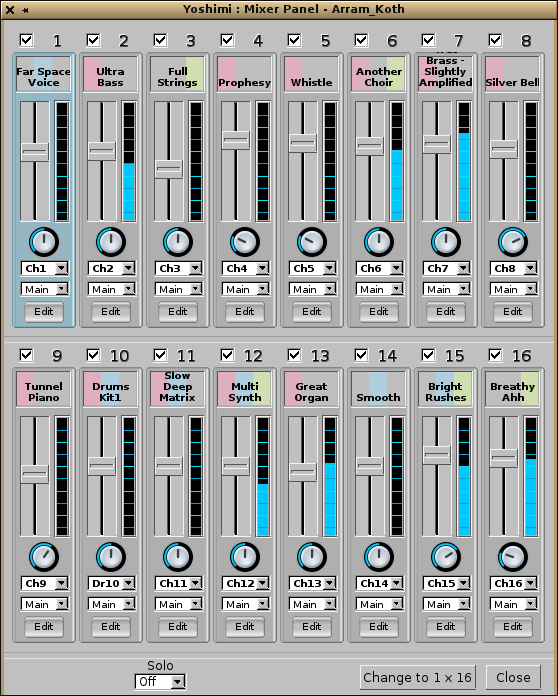
\includegraphics[scale=0.75]{1.5.0/Mixer8.png}
   \caption[Yoshimi Mixer Panel]{Yoshimi Mixer Panel, 2x8 View}
   \label{fig:yoshimi_part_panel_2x8}
\end{figure}

   Note that there is also a 1x16 version of this dialog (not shown).
   This dialog has been updated recently; there is now a \textbf{Solo}
   control, described below.

   \setcounter{ItemCounter}{0}      % Reset the ItemCounter for this list.

   \itempar{Part Summary}{Part Section, 1 to 16}
   Parts View or Summary.

   \itempar{Enable part}{parts!enable}
   Enable/Disable the part. The check-box enables/disables the part.
   When the part is disabled, its controls are greyed out.

   Values: \texttt{Off*, On}

   \itempar{Part name}{parts!name}
   Instrument name. Click on this box to change the instrument (it will
   open up the \textbf{Edit} window.

   \itempar{Volume Slider}{parts!volume}
   Volume Bar.
   Changes the volume of the part.

   \itempar{VU-meter display}{parts!meter}
   Shows the level of the part when playing.

   \itempar{Panning Knob}{parts!panning}
   Panning Dial-Button.
   Changes the panning of the part.

   Values: \texttt{0 (left) to 64* (center) to 127 (right)}

   \itempar{Channel}{parts!channel}
   Receive from MIDI channel.
   Changes the MIDI channel assigned to the part.

   Values: \texttt{Ch1*, Ch2, ..., Ch16}

   \itempar{Main}{parts!destination}
   Set Audio Destination.
   Sets the audio for this part to be routed to the main audio output, to
   the audio specified by the part setup, or to both outputs.
   This option requires that \textsl{Yoshimi} use JACK audio.  If running
   ALSA, this option is disabled (greyed out).
   The part's audio destination (JACK) is saved with the parameter sets, and
   so is the number of available parts.  (\textsl{ZynAddSubFX} will still
   load these files, but it ignores any settings it doesn't recognise. If
   one re-saves in \textsl{ZynAddSubFX}, the settings will be lost.)

   Values: \texttt{Main, Part, or Both}

   \itempar{Edit}{parts!edit}
   The Edit button provides two function
   Left mouse button: Part select.
   Right mouse button: Instrument edit.
   This setup is a bit unintuitive, but the tooltips make it clear
   which click one might want to use.

   \itempar{Solo}{parts!solo}
   \index{channel switcher}
   \index{parts!channel switcher}
   There are two commands that change the way
   \textsl{Yoshimi} responds to incoming MIDI,
   so that only one of a group of instruments will see note-on events, but all
   of the group will see note-off ones. These commands
   are both in the \textbf{Mixer Panel}.

   They are referred as a \textsl{Solo} feature or a \textsl{Channel Mixer}
   feature.  The \textbf{Solo} settings are saved in patch sets, which saves a
   little frustration when loading one's current favorite patch set.

   Values: \texttt{Off*, Row, Col, Loop}

   For these modes, if one has a programmable MIDI controller, one can set it
   up to activate a specific part, or to increment/decrement which part in the
   set is active.  The \textbf{Solo} drop-down list enables the feature for
   either \textbf{Row} or \textbf{Col}umn mode, and also makes the CC spin-box
   visible.

   One uses this spin-box to set which incoming CC changes the part that gets
   new notes.
   The \textsl{value} this CC sends performs the actual change, instantly and
   silently. Most importantly it leaves any existing notes sounding through a
   note off release and the effects tail.

   \index{solo!row}
   \textbf{Row} means that all of the first 16 channels will be set to channel
   1, but with only one active, and one's CC will dial up any of the parts,
   disabling the others.
   In \textbf{Row} mode the whole of the first 16 parts are ostensibly
   receiving on channel 1.  This mode is most useful if one wants to play live
   through a piece with multiple instrument changes while playing. It works
   best with a foot switch that internally stores a channel number and
   increments/decrements it with every press, then sends it.

   Although this uses all of the first 16 parts, one can set the number of
   parts to 32, so that one can use the 17+ row for normal 1 through 16
   channels. Also, if one has \textbf{vector control} set up, \textbf{Solo}
   intelligently recognises this fact, and, for each vector it finds, it will
   switch in/out the whole vector column appropriately.

   \index{solo!column}
   For running \textbf{Solo} in \textbf{Column} mode, one needs to have 32 or
   (preferably) 64 parts set; with this setup, one can have up to 4 parts
   switched per channel, and independently of each other. However, this works
   more like vector control in that you have to switch in groups of 16. For
   example, to control the channel 4 column one would send 4, 20, 36, 52 to
   select the wanted part. This usage is more appropriate for post recording
   MIDI automation.

   For both of these modes, if one has a programmable MIDI controller, one can
   set it up to activate a specific part, or the increment/decrement which part
   in the set is active.

   \index{solo!loop}
   \textbf{Loop}.  Loop mode is a variation on the Row mode.
   With this mode, if one sends \textsl{any} value (except zero)
   via the designated CC,
   it will increment the active part by one, rolling round to 1 after 16.
   This should make even the dumbest foot controller usable.

   To keep it all lightweight, one needs to load and activate all the patches
   and parts wanted, but that could be obtained from a saved patch set, and the
   channels are only changed from the very first time one sends the CC.  To look
   really clever, the whole lot can be embedded in a MIDI file.

   One can play a piece that needs to live-switch between 10 instruments, using
   a footswitch to do the channel changes. The device holds a channel
   number (starting with zero) and increments/decrements it depending on which
   switch is pressed, then sends the resulting CC.

   \itempar{Parts Layout}{parts!change layout}
   \index{parts!2x8}
   \index{parts!1x16}
   Changes the layout of the panel to the other layout, either
   \textbf{Change to 2 x 8} or
   \textbf{Change to 1 x 16}.

   \itempar{Close}{parts!close}
   Close the window.

\subsection{Virtual Keyboard}
\label{subsec:virtual_keyboard}

   This section describes the detailed usage of the
   \textsl{Yoshimi} virtual keyboard.
   The virtual keyboard lets one play notes using the keyboard/mouse. There is
   no MIDI requirement. 
    
   Using the computer keyboard: The keyboard is split into two "octaves" (in
   fact it is more than 1 octave). It may happen that the keys will not trigger
   any note-on. This is because another widget than the keyboard itself is
   selected.  In order to continue playing using the keyboard, click with the
   mouse on some keys on the virtual keyboard, to give it computer keyboard
   focus.
   
   Using the mouse: One can use the mouse too, to play.  If one presses the
   shift key while pressing the mouse button, the keys will be not released
   when the mouse button is released.  If one presses the \textbf{Stop!} or
   "panic" button from the \textsl{ZynAddSubFX}/\textsl{Yoshimi} main window,
   all keys are released. 

\begin{figure}[H]
   \centering 
%  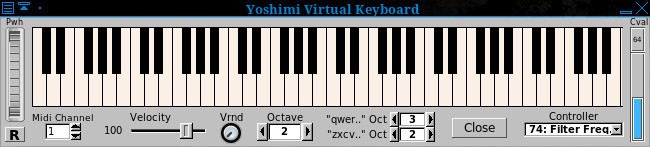
\includegraphics[scale=1.0]{top-panel/yoshimi-virtual-keyboard.jpg}
   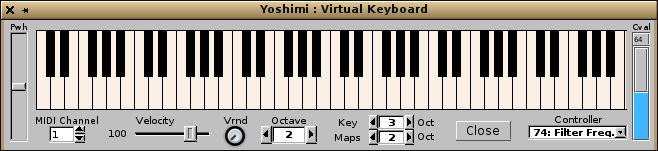
\includegraphics[scale=1.0]{1.5.0/Keyboard.png}
   \caption{Yoshimi Virtual Keyboard}
   \label{fig:yoshimi_virtual_keyboard}
\end{figure}

\subsubsection{Virtual Keyboard, Basics}
\label{subsubsec:virtual_keyboard_basics}

   \begin{enumber}
      \item \textbf{Pwh}
%     \item \textbf{R}
      \item \textbf{Midi Channel}
      \item \textbf{Velocity}
      \item \textbf{Velocity}
      \item \textbf{Octave}
      \item \textbf{Key Oct}
      \item \textbf{Maps Oct}
      \item \textbf{Controller}
      \item \textbf{Cval}
      \item \textbf{Close}
   \end{enumber}

   \itempar{Pwh}{vkdb!pitch bend}
   Pitch bend knob. Pitch wheel.
   This item is now a slider control.  To reset it to the middle position,
   right-click within the slider.

%  Press the \textbf{R} button to reset it.
%
%  \itempar{R}{vkdb!reset pitch bend}
%  Reset Pitch Bend.

   \itempar{Midi Channel}{vkdb!midi channel}
   MIDI Channel.
   Sets the MIDI channel for the virtual keyboard.

   Values: \texttt{1* to 16}

   \itempar{Velocity}{vkdb!velocity}
   Velocity of Notes.
   Sets the note-on velocity for the virtual keyboard.

   Values: \texttt{1 to 127, 100*}

   \itempar{Velocity}{vkdb!velocity randomness}
   Velocity Randomness.

   Values: \texttt{0* to 127}

   \itempar{Octave}{vkdb!qwerty}
   Transposes all of the virtual keyboard notes by the given number of
   octaves.

   Values: \texttt{1, 2*, 3, 4, 5}

%  \itempar{"qwer.." Oct}{vkdb!qwert}
%  q2w3e4r5t6y Octave.

   \itempar{Key Oct}{vkdb!key octave}
   Transposes the upper keys (the numbers and the "qwert" keys);
   the range of these keys is from C-4 to A-5 (replace the '5' with the octave).
   Look at the tooltips as a reminder.

   Values: \texttt{1, 2*, 3, 4, 5}

%  \itempar{"qwer.." Oct}{vkdb!zxcvb}
%  zsxdcfvgbh Octave.

   \itempar{Maps Oct}{vkdb!maps octave}
   Transposes the lower keys ("sdghj" and "zxcvb"); the range of these keys is
   from C-3 to E-4 (replace the '4' with the octave).  Look at the tooltips as a
   reminder.

   Values: \texttt{1, 2*, 3, 4, 5}

   \itempar{Controller}{vkdb!controller}
   Keyboard Controller.

   Values: \texttt{01:Mod.Wheel, 07:Volume, 10:Panning,
      11:Expression, 64:Sustain, 65:Portamento, 71:Filter Q,
      74:Filter Freq*, 75:Bandwidth, 76:FM Gain,
      77:Res.c.freq, 78:Res.bw.}

   Sets the controller to be changed according to the \textbf{Cval}
   controller.
   See \sectionref{subsubsec:virtual_keyboard_controllers}.

   \itempar{Cval}{vkdb!controller value}
   Controller value.
   Changes the controller value.
   This item consists of two parts.  The top part shows a tiny
   number representing the current value of the selected controller.
   The bottom part is a combination value-bar and slider that one
   can move up and down with the mouse, to change the controller value.
   Note that the \textbf{Cval} value might not reflect the
   internal value of the controller when one changes the controller.

   Values: \texttt{1 to 127, 96*}

   \itempar{Close}{vkdb!close}
   Close button.

\subsubsection{Virtual Keyboard, ASCII Mapping}
\label{subsubsec:virtual_keyboard_ascii}

   In addition to this virtual keyboard, the QWERTY (or Dvorak, or AZERTY)
   keyboards can be used to produce notes.
   The computer keyboard layout is shown in
   \figureref{fig:qwerty_virtual_keyboard},
   From lowest octave to highest, the colors are blue, then green, then red.
   The "white" keys are the light colors, and the "black" keys are the
   deeper colors.
   The range of the keys on the "zxcvb..." row is C3 to E4.
   The range of the keys on the "qwert..." row is C4 to A5.
   These octave ranges can be adjusted.

   The computer keyboard will produce notes only when the virtual keyboard
   is active.
   Also note that we replaced the monopoly symbol with the monopolist
   symbol.  On X11 systems, this key is known as the "Super" key.

\subsubsection{Virtual Keyboard, Controllers}
\label{subsubsec:virtual_keyboard_controllers}

   This section (will give) a brief overview of the controller's that this
   window supports.

   \begin{enumber}
      \item \textbf{01: Mod. Wheel}
      \item \textbf{07: Volume}
      \item \textbf{10: Panning}
      \item \textbf{11: Expression}
      \item \textbf{64: Sustain}
      \item \textbf{65: Portamento}
      \item \textbf{71: Filter Q}
      \item \textbf{74: Filter Freq.}
      \item \textbf{75: Bandwidth}
      \item \textbf{76: FM Gain}
      \item \textbf{77: Res. c. freq}
      \item \textbf{78: Res. bw.}
   \end{enumber}

      The following figure shows the corresponding drop-down list of controller
      values, each preceded by its MIDI control number, re 1.

\begin{figure}[H]
   \centering 
%  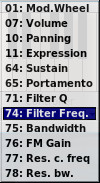
\includegraphics[scale=0.75]{menu/Instrument/virtual-keyboard-controllers.jpg}
   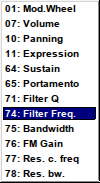
\includegraphics[scale=0.75]{top-panel/virtual-keyboard-controller.png}
   \caption{Virtual Keyboard Controllers}
   \label{fig:virtual_keyboard_controllers}
\end{figure}

   \setcounter{ItemCounter}{0}      % Reset the ItemCounter for this list.

   \itempar{Mod. Wheel}{controllers!modulation wheel}
   Sets the MIDI modulation value.  This control will
   only have an effect on certain instruments.  (It has no effect on the
   "Simple Sound", for example).

   \itempar{Volume}{controllers!volume}
   Controls the overall volume of the instrument being played by the virtual
   keyboard.

   \itempar{Panning}{controllers!panning}
   Controls the left-right location of the sounds played by the virtual
   keyboard.

   \itempar{Expression}{controllers!expression}
   Controls the expression.  This probably can have different effects depending
   on the instrument.  For example, with the "Simple Sound", this control is a
   lot like volume.

   \itempar{Sustain}{controllers!sustain}
   Controls the sustain duration.  This works even with the "Simple Sound".
   Using it makes even this virtual keyboard capable of some "virtuoso"
   expression.

   \itempar{Portamento}{controllers!portamento}
   Controls the time of transition from one pitch to another.
   Using it makes even this virtual keyboard capable of some "virtuoso"
   expression.

   \itempar{Filter Q}{controllers!filter q}
   Controls the sharpness of the filters used in an instrument.
   Generally requires a complex instrument to take effect.
   For example, try this control with the "Weird Pad" instrument in the
   "Fantasy" bank.

   \itempar{Filter Freq}{controllers!filter frequency}
   Controls the center frequency of the filters used in an instrument.
   Generally requires a complex instrument to take effect.
   For example, try this control with the "Weird Pad" instrument in the
   "Fantasy" bank.

   \itempar{Bandwidth}{controllers!bandwidth}
   Controls the frequency bandwidth of the filters used in an instrument.

   \itempar{FM Gain}{controllers!fm gain}
   TODO.
   Haven't found a sound that exercises this control.
   Haven't looked all that hard yet.

   \itempar{Res. c. freq}{controllers!resonant center frequency}
   TODO.
   Not sure how this differs from \textbf{Filter Freq.}.
   Haven't found a sound that exercises this control.
   Haven't looked all that hard yet.

   \itempar{Res. bw}{controllers!resonant bandwidth}
   TODO.
   Not sure how this differs from \textbf{Bandwidth}.
   Haven't found a sound that exercises this control.
   Haven't looked all that hard yet.

%-------------------------------------------------------------------------------
% vim: ts=3 sw=3 et ft=tex
%-------------------------------------------------------------------------------
